\mkexercise{El amplificador de la figura se encuentra polarizado con
  una pila de 5 $V$, una red de realimentación en corriente y
  configurado en \textbf{Colector Común} con un transistor tipo
  Q2N3904(bipolar.lib), una $\beta_{DC} = 103$, una $\beta_{AC}=70.3$, una
tensión base-emisor $V_{BE}=0.8 V$, una tensión Early $V_{AF}=74.03 V$
y una tensión térmica a $27^{\circ}$ de $V_T=25.85 mV$. La carg $RL =
10+(DNI \cdot 0.005) \Omega$ ajustada a dos decimales, donde
\textit{DNI} se corresponde con las tres cifras menos significativas
del \textit{DNI} o documento acreditativo.

\begin{itemize}
  \item Calcular analíticamente las tensiones en los nodes y las
    corrientes que circulan por la red de polarización, verificando
    los resultados mediante simulación ``bias point''.
  \item Calcular analíticamente los parámetros del amplificador:
    Ganancia en Tensión $A_V$, Ganancia en Corriente $A_I$, impedancia
    de Entrada $Z_{in}$, e impedancia de Salida $Z_{zout}$, medidos a
    frecuencias intermedias utilizando la resistencia Rl con el valor
    definido en el enunciado.
    \item Verificar los parámetros del amplificador calculados
      analíticamente mediante simulación.
  \end{itemize}

}

  \begin{figure}[H]
    \centering  
    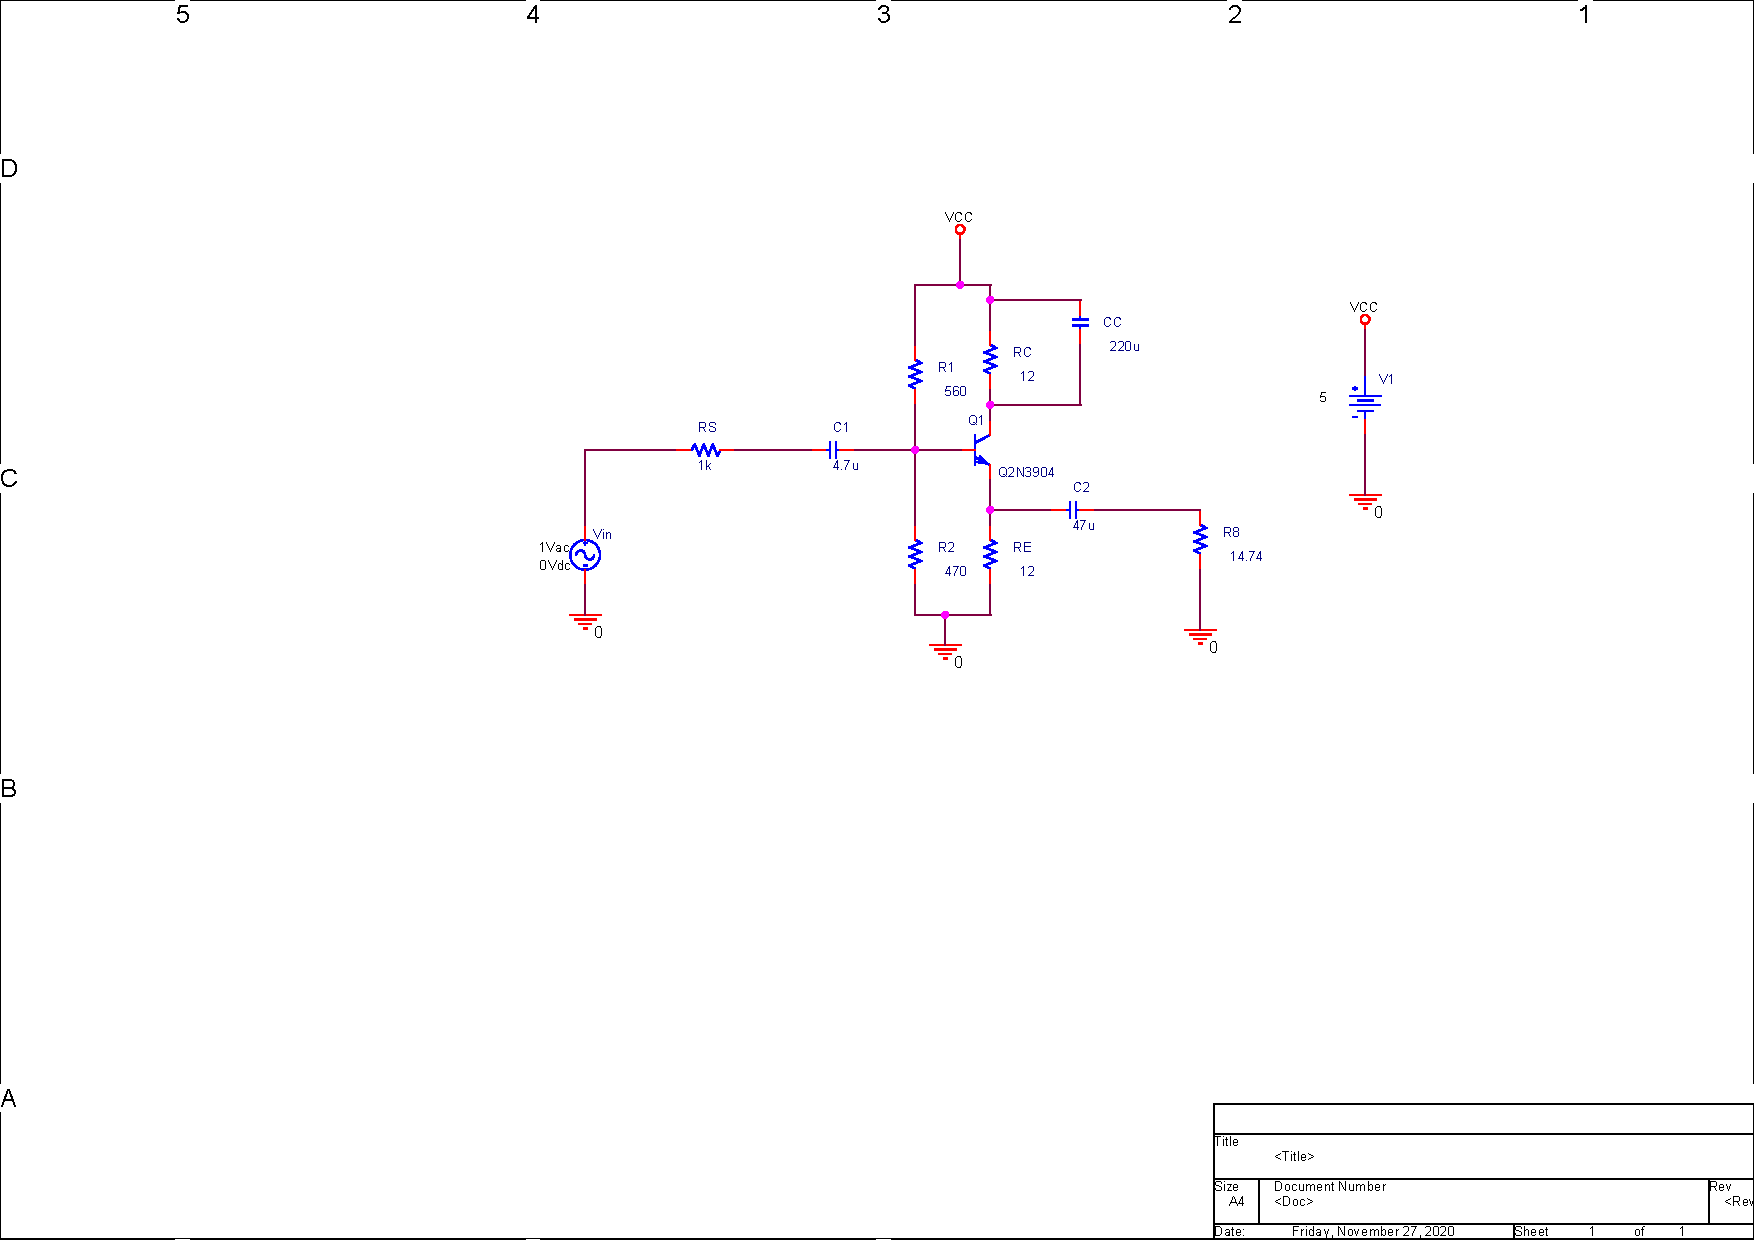
\includegraphics[scale=1,page=1,clip, trim=8cm 9.5cm 5cm 3.5cm]{images/circuito_completo.pdf}
    % izquierda,abajo,derecha,arriba
    \caption{Amplificador esquema}
  \end{figure}

Para analizar la polarización del circuito tenemos que calcular el
equivalente thévenin en la base del transistor. Desconectamos la carga
y calculamos $V_{TH}$ y $R_{TH}$.

  \begin{figure}[H]
    \centering  
    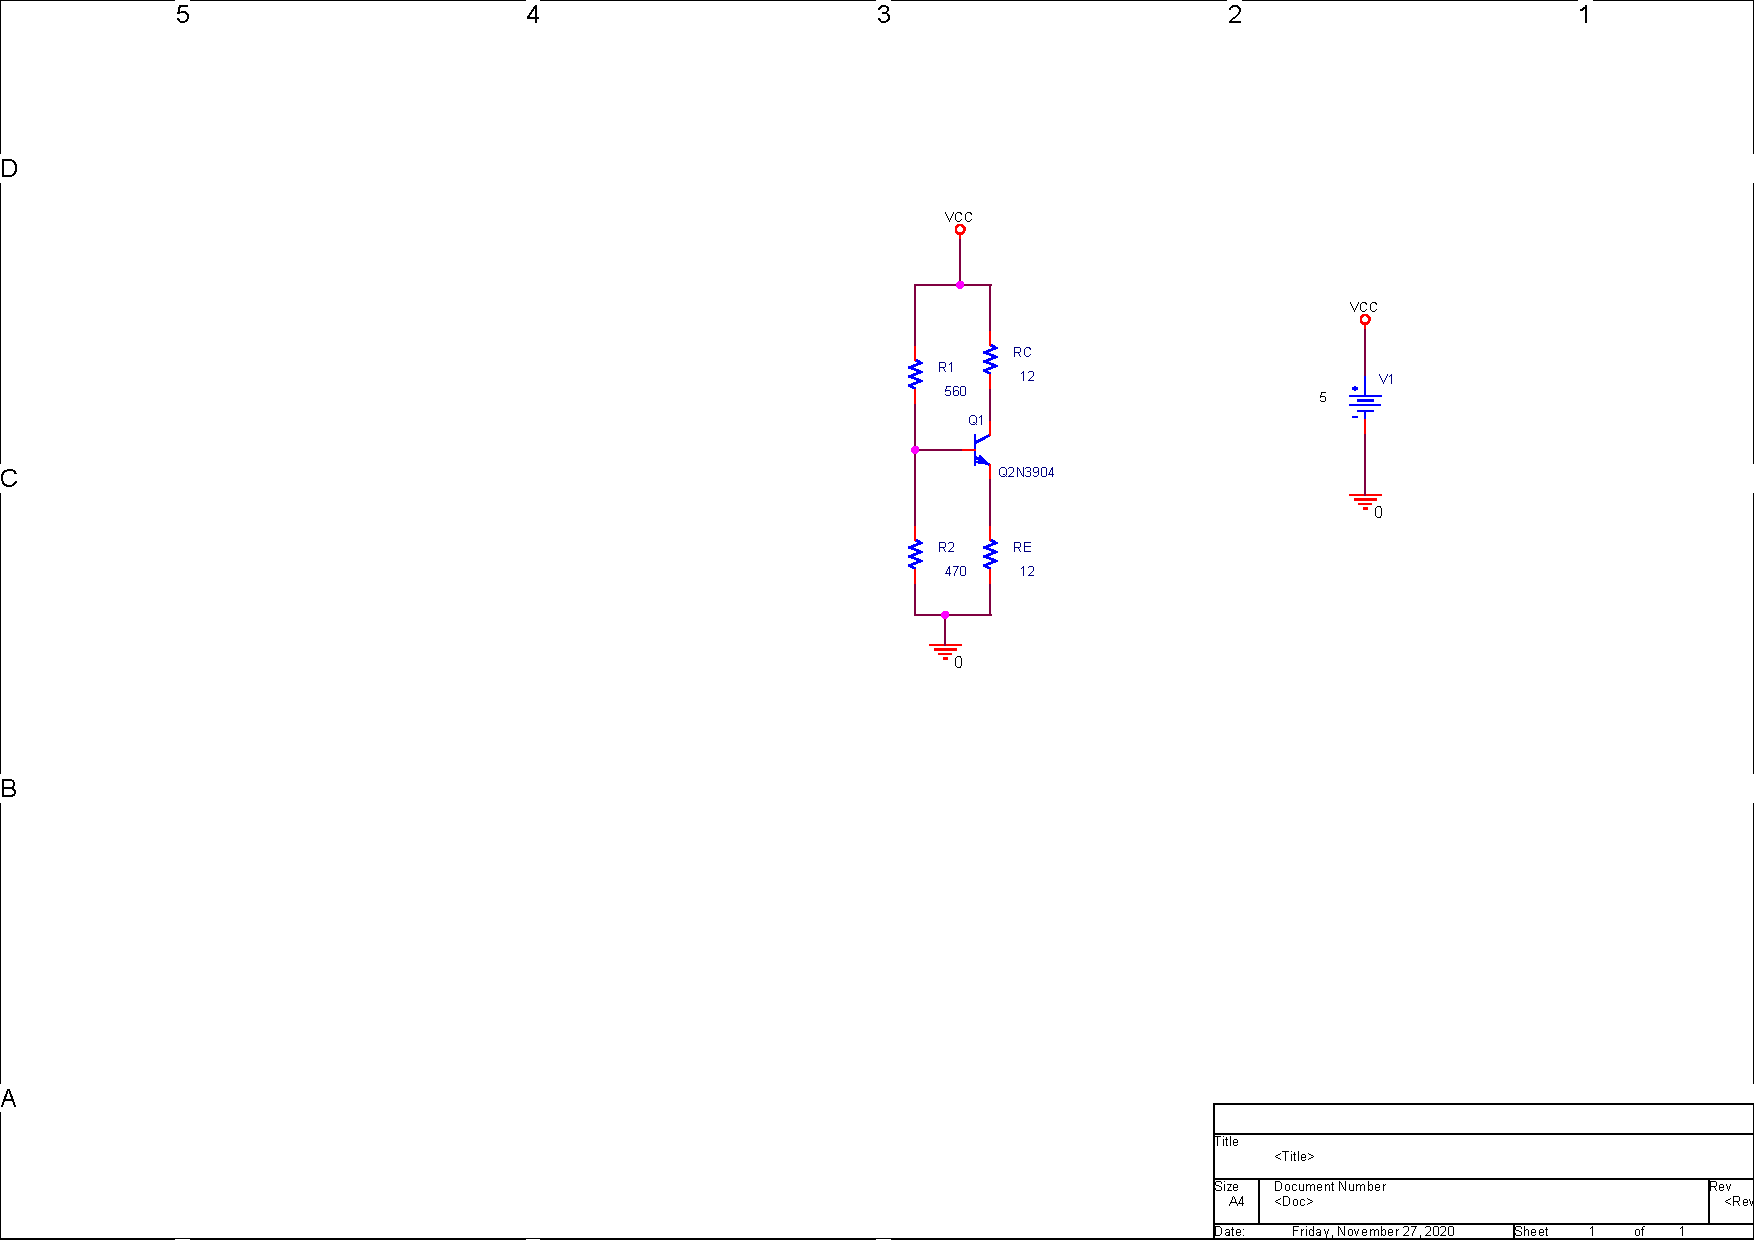
\includegraphics[scale=1,page=1,clip, trim=8cm 9.5cm 5cm 3.5cm]{images/circuito_sin_bias_point.pdf}
    % izquierda,abajo,derecha,arriba
    \caption{Circuito de polarización}
  \end{figure}

Calculamos $V_{TH}$:
\begin{equation}
  \begin{split}
    0 &= Vcc - iR_1-iR_2\\
    V_B &= iR_2\\
    Vcc &= V_B\left(\dfrac{R1+R2}{R2}\right)\\
    V_B &= \dfrac{Vcc \cdot R_2}{R_1+R_2}\\
    V_B &= \dfrac{5 \cdot 470}{470+560} = 2.281 V
  \end{split}
\end{equation}

Calculamos $R_{TH}$:
Las fuentes de tensión se transforman en un cortocircuito y el
equivalente en un paralelo.
\begin{equation}
  \begin{split}
    R_{TH} &= \dfrac{1}{\dfrac{1}{R_1}+\dfrac{1}{R_2}}\\
    R_{TH} &= \dfrac{1}{\dfrac{1}{560}+\dfrac{1}{470}}\\
    R_{TH} &= 255.53 \Omega
  \end{split}
\end{equation}

Por seguir una notación fija durante todo el problema $V_{TH}$ será
$V_B$ y $R_{TH}$ será $RB$.

Generamos el sistema de ecuaciones con el que vamos a trabajar para
hallar $I_C,I_B,I_E$, $V_c,V_E,V_B$, $V_{CE},V_{CB}$.

\begin{equation}
  \left \{
    \begin{split}
      I_E & = I_C+I_B\\
      0 & = Vcc - i_cRC-V_{CE}-i_eRE\\
      0 & = V_B-i_bRB-V_{BE}-i_ERE\\
    \end{split}
  \right.
\end{equation}

\begin{equation}
    \begin{split}
      \beta & = \dfrac{I_c}{I_B}\\
      I_E & = \beta_{DC} I_B + I_B\\
      I_E & = I_B(\beta +1)\\
      0 & = Vcc +\beta_{DC} I_BRC-V_{CE}-I_B(\beta_{DC}+1)RE\\
      0 & = V_B-I_BRB-V_{BE}-I_B(\beta_{DC}+1)RE\\
      V_B-V_{BE} & =I_BRB+I_B(\beta_{DC}+1)RE\\
      I_B & = \dfrac{V_B-V_{BE}}{RB+(\beta_{DC}+1)RE}
    \end{split}
  \end{equation}

  \begin{equation}
    \begin{split}
      I_B & = \dfrac{I_C}{\beta_{DC}}\\
      I_E & = \dfrac{\beta_{DC} I_C}{\beta_{DC}} +\dfrac{I_C}{\beta_{DC}}\\
      I_E & = \dfrac{I_C(1+\beta_{DC})}{\beta_{DC}}\\
      0 & = V_B-I_BRB-V_{BE}-I_ERE\\
      0 & = V_B-\dfrac{I_C}{\beta_{DC}}RB-V_{BE}-\dfrac{I_C(1+\beta_{DC})}{\beta_{DC}}RE\\
      I_C & = \dfrac{V_B-V_{BE}}{\dfrac{RB}{\beta_{DC}}+\dfrac{RE(1+\beta_{DC})}{\beta_{DC}}}\\
     \end{split}
   \end{equation}

    Si $\beta$ es lo suficientemente grande podemos aproximar $I_C$ como:
    \[I_C  = \dfrac{V_B-V_{BE}}{\dfrac{RB}{\beta_{DC}}+RE}\]
    
  \begin{equation}
      V_{CE} = Vcc-\left(\dfrac{V_B-V_{BE}}{RB+(\beta_{DC}+1)RE}\right)RE\beta_{DC}-\left(\dfrac{V_B-V_{BE}}{RB+(\beta_{DC}+1)RE}\right)(\beta_{DC}+1)RE
    \end{equation}

    En resumen:
    Corrientes en los terminales del transistor:
\begin{equation}
  \begin{split}
    I_B & = \dfrac{2.281-0.8}{255.53+(103+1)12}\\
    I_B & = 985 \ \mu A\\
    I_C & = \dfrac{2.281-0.8}{\dfrac{255.53}{103}+12}\\
    I_C & = 102.27 \  mA\\
    I_E & = 0.985 + 102.27\\
    I_E & = 103.255 \  mA
  \end{split}
\end{equation}

Tensiones en los terminales del transistor:

\begin{equation}
  \begin{split}
    V_E & =I_E(RE)\\
    V_E & =103.25 \ mA(12 \Omega)\\
    V_E & = 1.239 \ V\\
    V_C & =Vcc-I_CRC\\
    V_C & =5-(102.27 \ mA)(12 \Omega)\\
    V_C & = 3.773 \ V\\
    V_B & =V_E+V_{BE}\\
    V_B & = 1.239 + 0.8\\
    V_B & = 2.039 \ V
  \end{split}
\end{equation}

Valores extra:

Se debe considerar que $V_B$ no es la tensión Thévenin calculada en el
primer apartado, es la tensión en la base del transistor. Este cambio
se produce porque estamos considerando toda la red de polarización no
solo la caída de tensión en el nudo B.

\begin{equation}
  \begin{split}
    I_{R1} & = \dfrac{Vcc-V_B}{R1}\\
    I_{R1} & = \dfrac{5-2.039}{560}\\
    I_{R1} & = 5.28 \ mA \\
    I_{R2} & = \dfrac{V_B}{R2} \\
    I_{R2} & = \dfrac{2.039}{470}\\
    I_{R2} & = 4.34 \ mA
  \end{split}
\end{equation}

Con los datos anteriores podemos calcular todas las potencias de los
elementos e incluso la del transistor:

\[W_{BJT} = I_E\cdot V_{CE}=I_E\cdot (V_C-V_E) = \mili{103.255}\cdot (3.773 -
  1.239) = 257 mW\]


%% Insertar imagen bias point''

Como podemos observar en el simulador las tensiones y corrientes
calculadas analíticamente son muy próximas y en la siguiente tabla
podemos observar la dispersión que hay entre los resultados.

\begin{center}
\begin{tabular}{| c | c | c | c |}
\hline
Variable & Analítico & Simulación  & Dispersión\\ \hline
  $I_B$ & 985 $\mu A$ & 975.4 $\mu A$ & 1\%\\
  $I_C$ & 102.27 $mA$ & 100.3 $mA$ & 1.92\%\\
  $I_E$ & 103.255 $mA$ & 101.3 $mA$ & 1.89\%\\
  $V_E$ & 1.239 $V$ & 1.215 $V$ & 1.94\%\\
  $V_C$ & 3.773 $V$ & 3.796 $V$ & 0.61\%\\
  $V_B$ & 2.039 $V$ & 2.032 $V$ & 0.34\% \\
  $I_{R1}$ & 5.28 $mA$ & 5.299 $mA$ & 0.35\%\\
  $I_{R2}$ & 4.34 $mA$ & 4.324 $mA$ & 0.37\%\\ \hline
\end{tabular}
\end{center}

  \begin{figure}[H]
    \centering  
    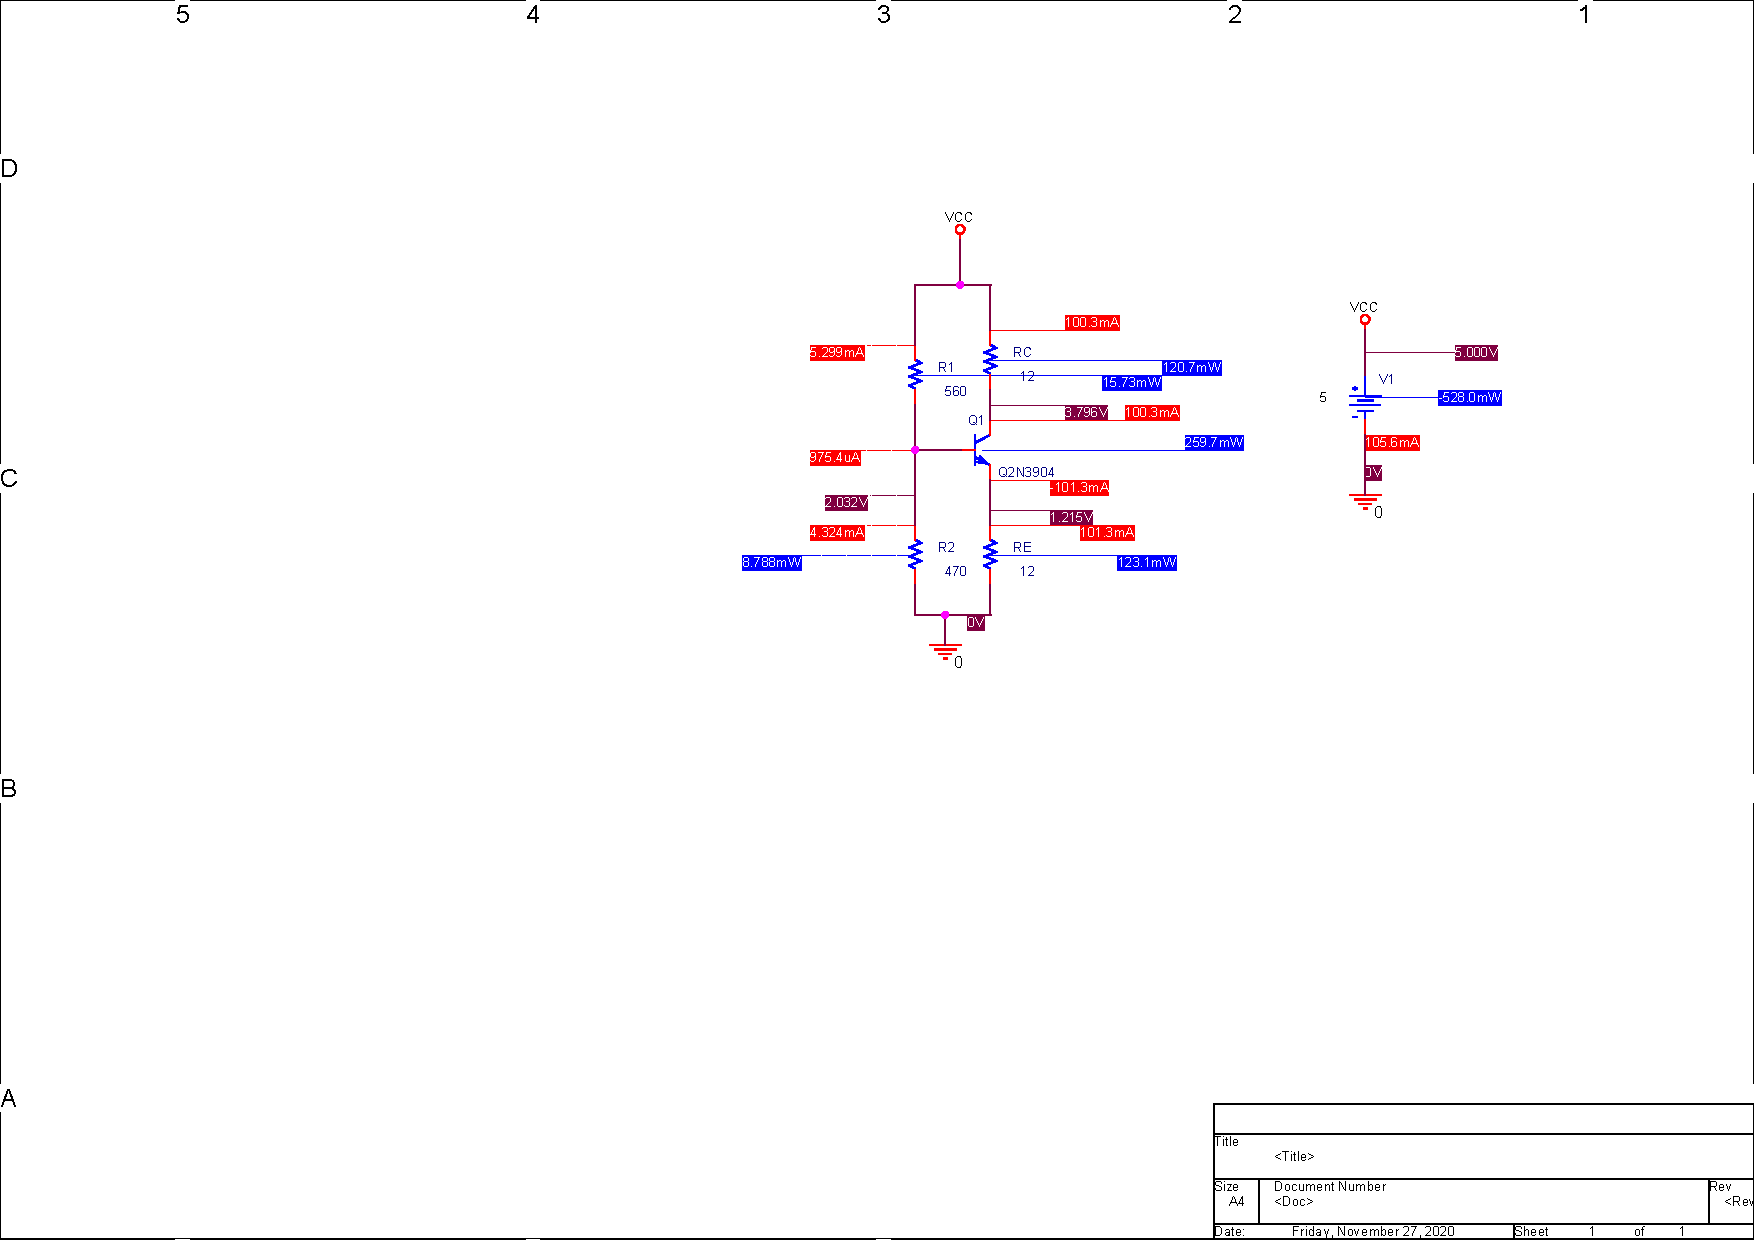
\includegraphics[scale=1,page=1,clip, trim=10cm 9.5cm 3cm 3cm]{images/circuito_bias_point.pdf}
    % izquierda,abajo,derecha,arriba
    \caption{Bias point al circuito de polarización}
  \end{figure}

Análisis analítico:
\begin{itemize}
\item \textbf{Estimación de la transconductancia GM}
  \[GM = \dfrac{I_C}{V_T} = \dfrac{102.27 mA}{25.85 mV} = 3.95\]
\item \textbf{Estimación de la resistencia RPI}
  \[RPI = \dfrac{\beta_{AC}}{GM} = \dfrac{70.3}{3.95} = 17.79 \Omega\]
  La resistencia de entrada cumple las necesidades de una ganacia en
  corriente, esta condición implica que la resistencia de entrada sea
  lo más baja posible.
\item \textbf{Estimación de la resistencia de salida RO}
  \[RO = \dfrac{R_{CE}+V_{AF}}{I_C} = \dfrac{2.53+74.03}{102.27 mA} =
    748.60 \Omega \]
  A diferencia de la RPI la resistencia de salida debe ser lo más alta
  posible para realizar la máxima amplificación y que la ganancia sea máxima.
\end{itemize}

Comparadas con la del simulador obtenemos diferencias bastante
significativas. Del orden del 55\% en algunos casos, es normal porque
nuestro modelo elimina muchos efectos de segundo y tercer orden,
nuestra primera aproximación se queda corta pero es útil desde el
punto educativo.

  \begin{figure}[H]
    \centering  
    \includegraphics[scale=1,page=3,clip, trim=0cm 10cm 23cm 5cm]{images/output.pdf}
    % izquierda,abajo,derecha,arriba
    \caption{Bias point al circuito de polarización}
  \end{figure}
  
\begin{itemize}
\item \textbf{Ganancia en Tensión}
  \begin{equation}
  \begin{split}
    A_V & = \dfrac{V_{out}}{V_{in}} \\
    A_V & = \dfrac{\dfrac{1}{\dfrac{1}{RE}+\dfrac{1}{RL}}}{\dfrac{RPI}{\beta_{AC}+1}+\dfrac{1}{\dfrac{1}{RE}+\dfrac{1}{RL}}}\\
    A_V & =
    \dfrac{\dfrac{1}{\dfrac{1}{12}+\dfrac{1}{14,74}}}{\dfrac{17.79}{70.3+1}+\dfrac{1}{\dfrac{1}{12}+\dfrac{1}{14.47}}}\\
    A_V & = 0.9636
  \end{split}
\end{equation}
Como era de esperarse la ganancia en tensión está cerca de la unidad,
ya que este amplificador está diseñado para amplificar la corriente luego es
normal que esté entorno a 1.
\item \textbf{Resistencia de Entrada}
  \begin{equation}
  \begin{split}
    R_{in} & =
    \dfrac{1}{\dfrac{1}{RB}+\dfrac{1}{\left(\dfrac{RPI}{\beta_{AC}+1}+\dfrac{1}{\dfrac{1}{RE}+\dfrac{1}{RL}}\right)
        \cdot (\beta_{AC}+1)}} \\
        R_{in} & = \dfrac{1}{\dfrac{1}{255.53}+\dfrac{1}{\left(\dfrac{17.79}{70.3+1}+\dfrac{1}{\dfrac{1}{12}+\dfrac{1}{14.74}}\right) \cdot (70.3+1)}} \\
    R_{in} & = 167.879 \Omega\\
  \end{split}
\end{equation}
Los amplificadores pueden tener un fallo en su función electrónica si la
impedancia de entrada es baja. Generalmente los circuitos
amplificadores con colector común tienen una impedancia de entrada
alta (comparada con la salida), si lo comparamos con la de salida el
circuito concuerda con la teoría.
\item \textbf{Resistencia de Salida }
    \begin{equation}
  \begin{split}
    R_{out} & = RE ||\left(
      \dfrac{RPI}{\beta_{AC}+1}+\left(\dfrac{RS||RB}{\beta_{AC}+1}\right)\right)\\
        R_{out} & = 12 ||\left( \dfrac{17.79}{70.3+1}+\left(\dfrac{1000||255.53}{70.3+1}\right)\right)\\
    R_{out} & = 2.466 \Omega\\
  \end{split}
\end{equation}

\item \textbf{Ganancia en Corriente}
    \begin{equation}
  \begin{split}
    A_I & = \dfrac{I_{out}}{I_{in}} \\
    A_I & = \dfrac{RE}{RE+RL} \cdot (\beta_{AC}+1) \cdot
    \dfrac{RB}{RB+(\dfrac{RPI}{\beta_{AC}+1}+RL||RE)\cdot
      (\beta_{AC}+1)}\\
    A_I & = \dfrac{12}{12+14.74} \cdot (70.3+1) \cdot
    \dfrac{255.53}{255.53+(\dfrac{17.79}{70.3+1}+14.74||12)\cdot (70.3+1)}\\
    A_I & = 10.97\\
  \end{split}
\end{equation}
Esta es la corriente que obtenemos del circuiot si en la entrada
metemos un 1mA, en la salida tendremos 10.97mA, el factor es proporcional.
\end{itemize}

Simulación:
\begin{itemize}
\item \textbf{Ganancia en Tensión}

  \begin{figure}[H]
    \centering  
    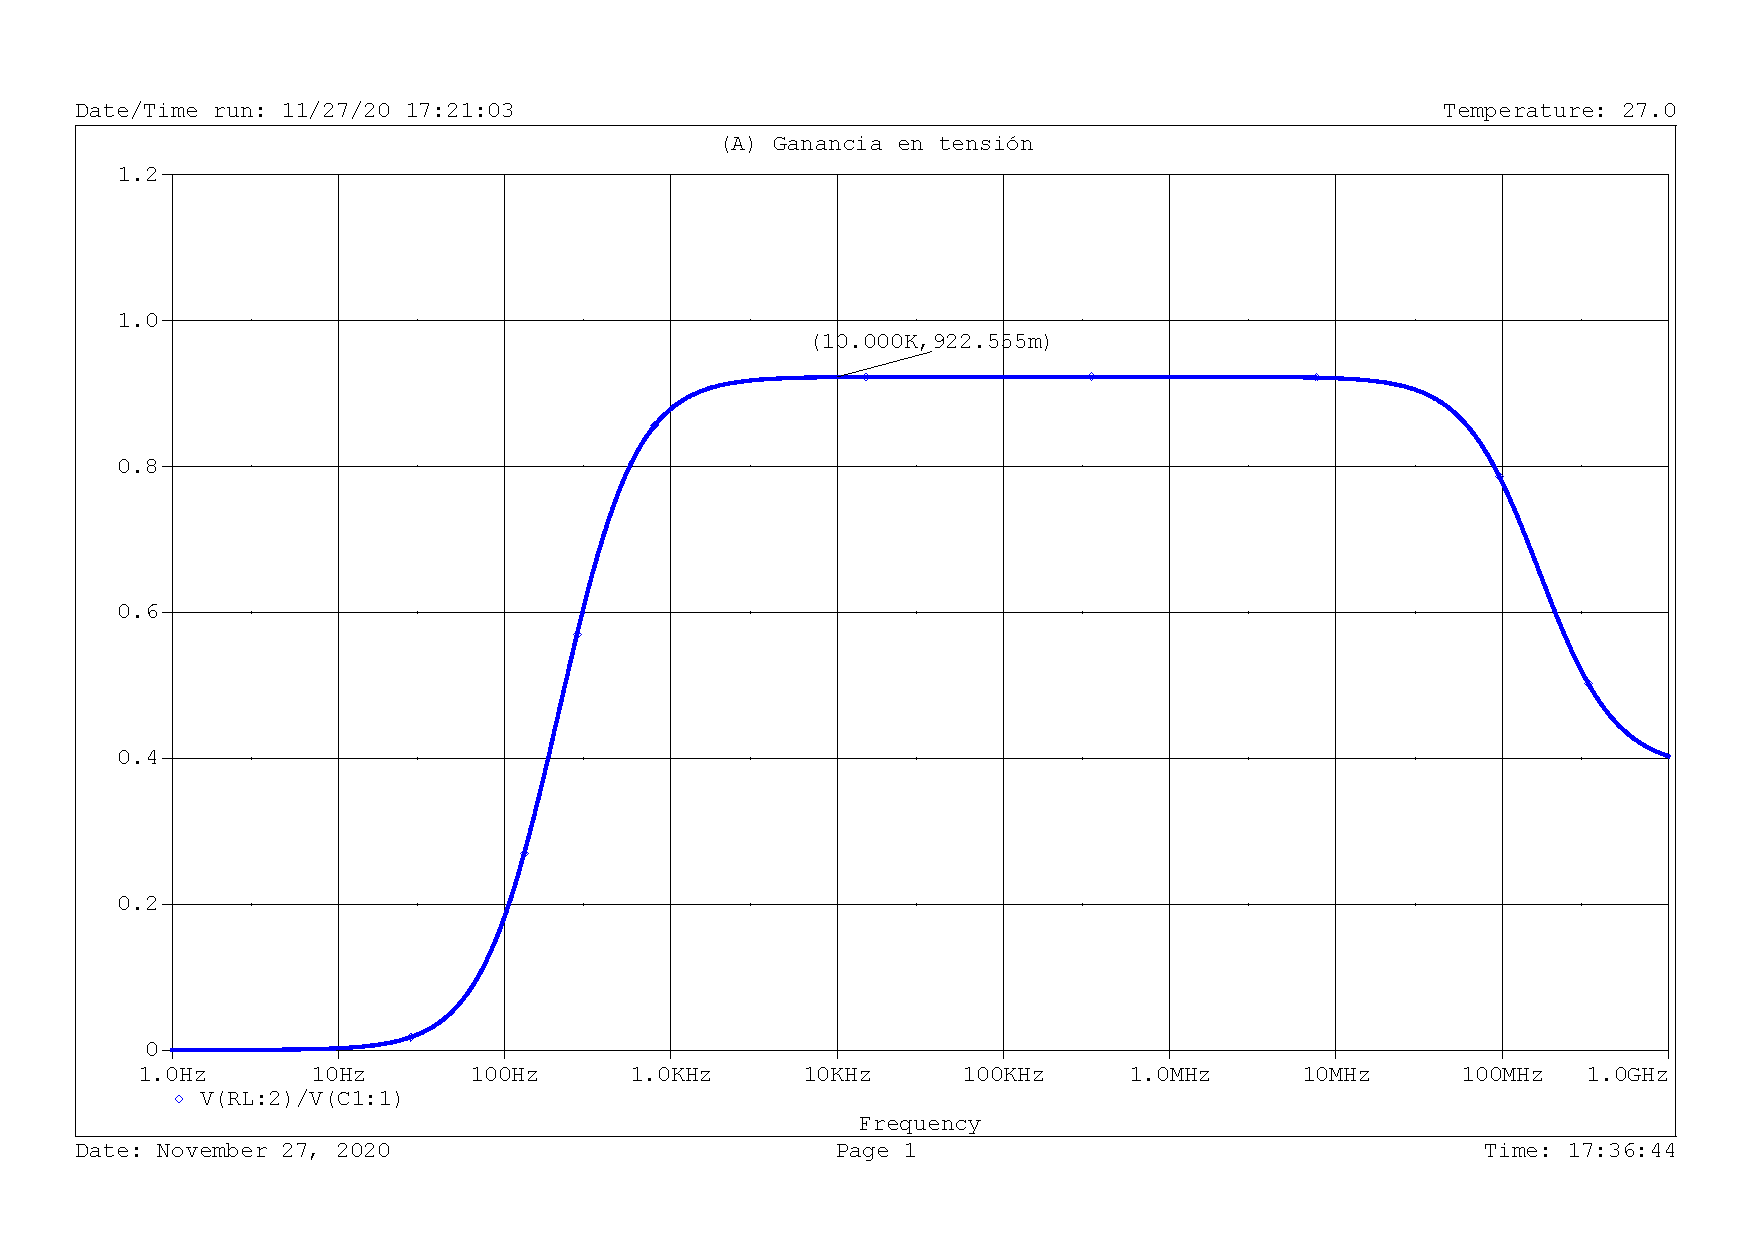
\includegraphics[scale=0.55,page=1,trim]{images/Amplificador_simulation.pdf}
    % izquierda,abajo,derecha,arriba
    \caption{Ganancia en tensión}                 
  \end{figure}
 Concuerda en gran medida con la ganancia obtenida en la parte
 analítica, podemos ver el rango de frencuencias en el que no hay
 distorsión que puede aproximarse con una recta.

\begin{figure}[H]
\centering  
\includegraphics[scale=0.55,page=2]{images/Amplificador_simulation.pdf}
% izquierda,abajo,derecha,arriba
\caption{Fase ganancia en tensión}
\end{figure}
En la fase observamos el mismo efecto en el que el aumento o
disminución de fase no es perceptible en ese rango de frecuencias.
\item \textbf{Ganancia en Corriente}
\begin{figure}[H]
\centering  
\includegraphics[scale=0.55,page=3]{images/Amplificador_simulation.pdf}
% izquierda,abajo,derecha,arriba
\caption{Ganancia en corriente}
\end{figure}
La ganacia en corriente obtenida en el apartado a se aproxima muy bien (para todas las
simplificaciones que hemos hechos) a la obtenida en el simulador, al
igual que la ganancia en tensión tiene un rango de frencuencias en el
que trabaja pero este es simétrico.

\begin{figure}[H]
\centering  
\includegraphics[scale=0.55,page=4]{images/Amplificador_simulation.pdf}
% izquierda,abajo,derecha,arriba
\caption{Fase ganancia en corriente}
\end{figure}
Mantiene la propiedad de recta de carga pero el rango es más pequeño.
\item \textbf{Resistencia de Entrada}
\begin{figure}[H]
\centering  
\includegraphics[scale=0.55,page=5]{images/Amplificador_simulation.pdf}
% izquierda,abajo,derecha,arriba
\caption{Impedancia de entrada}
\end{figure}
La impedancia de entrada está cerca de lo calculado analíticamente
para altas y medias frecuencias que es el rango de trabajo de nuestro
amplificador.
\item \textbf{Resistencia de Salida }
\begin{figure}[H]
\centering  
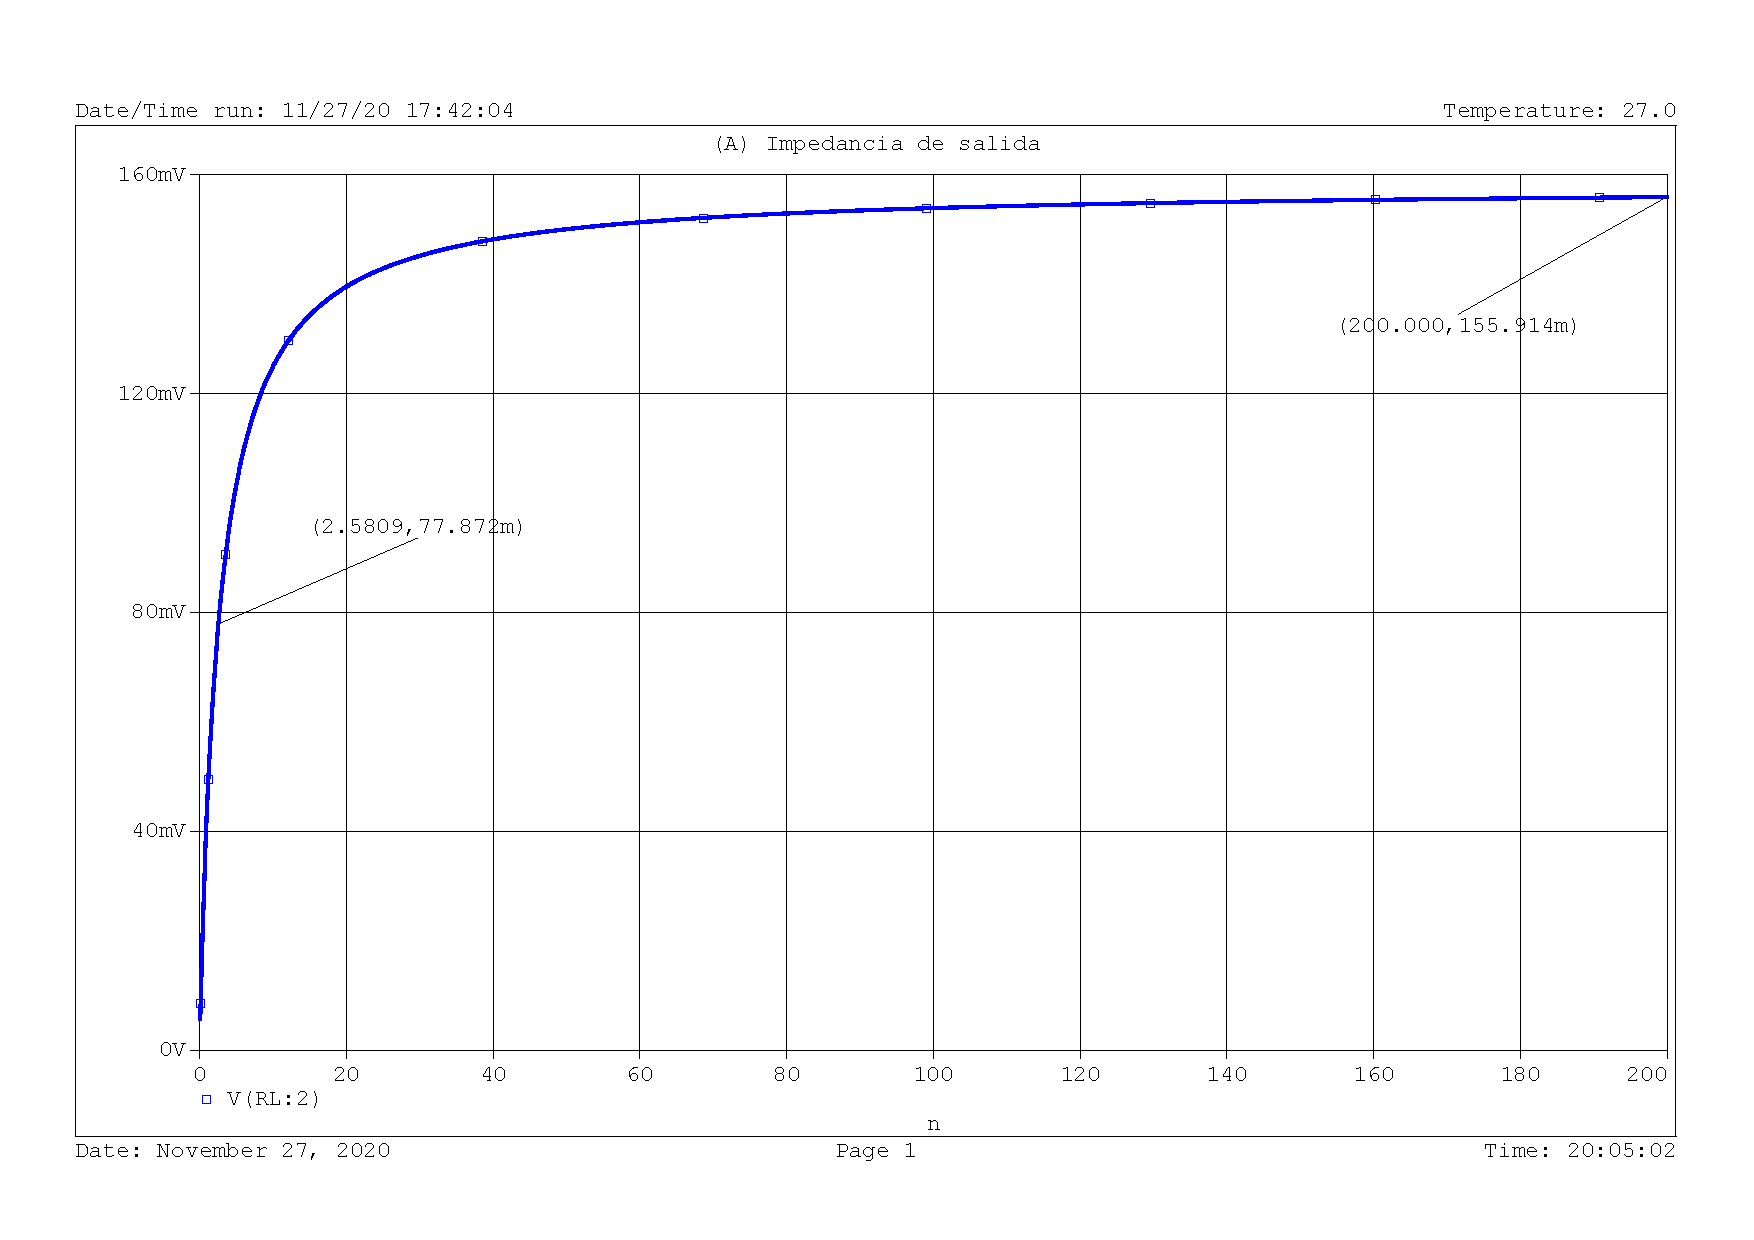
\includegraphics[scale=0.55,page=1]{images/Amplificador_simulation_last_part.pdf}
% izquierda,abajo,derecha,arriba
\caption{Impedancia de salida}
\end{figure}
En nuestra simulación no podemos ver el rango de frencuencias pero
podemos hacernos una idea por la forma que sigue la gráfica coincide
perfectamente con lo que hemos calculado analíticamente.
\item \textbf{Potencia del amplificador}
\begin{figure}[H]
\centering  
\includegraphics[scale=0.55,page=2]{images/Amplificador_simulation_last_part.pdf}
% izquierda,abajo,derecha,arriba
\caption{Potencia del amplificador}
\end{figure}

\end{itemize}

